%iffalse
\let\negmedspace\undefined
\let\negthickspace\undefined
\documentclass[journal,12pt,onecolumn]{IEEEtran}
\usepackage{cite}
\usepackage{amsmath,amssymb,amsfonts}
\usepackage{graphicx}
\usepackage{textcomp}
\usepackage{xcolor}
\usepackage{txfonts}
\usepackage{listings}
\usepackage{enumitem}
\usepackage{mathtools}
\usepackage{gensymb}
\usepackage{comment}
\usepackage[breaklinks=true]{hyperref}
\usepackage{tkz-euclide} 
\usepackage{listings}
\usepackage{gvv}                                        
\def\inputGnumericTable{}                                 
\usepackage[latin1]{inputenc}                                
\usepackage{color}                                            
\usepackage{array}                                            
\usepackage{longtable}                                       
\usepackage{calc}                                             
\usepackage{multirow}                                         
\usepackage{hhline}                                           
\usepackage{ifthen}                                           
\usepackage{lscape}
\usepackage[export]{adjustbox}
\newtheorem{theorem}{Theorem}[section]
\newtheorem{problem}{Problem}
\newtheorem{proposition}{Proposition}[section]
\newtheorem{lemma}{Lemma}[section]
\newtheorem{corollary}[theorem]{Corollary}
\newtheorem{example}{Example}[section]
\newtheorem{definition}[problem]{Definition}
\newcommand{\BEQA}{\begin{eqnarray}}
	\newcommand{\EEQA}{\end{eqnarray}}
\newcommand{\define}{\stackrel{\triangle}{=}}
\newtheorem{rem}{Remark}

\begin{document}
	\parindent 0px
	\bibliographystyle{IEEEtran}
	
	
	
	\title{}
	\author{EE23BTECH11209 - K S Ballvardhan$^{*}$
	}
	\maketitle
	\bigskip
	
	% \renewcommand{\thefigure}{\theenumi}
	% \renewcommand{\thetable}{\theenumi}
	
	
	
	
	\textbf{Question:} x[n] is convolved with h[n] to give y[n]. If y[2] = 1 and y[3] = 0 then find h[0]. (Graphs are not uniformly scaled) \hfill[GATE BM 2021]
	\begin{figure}[ht]
		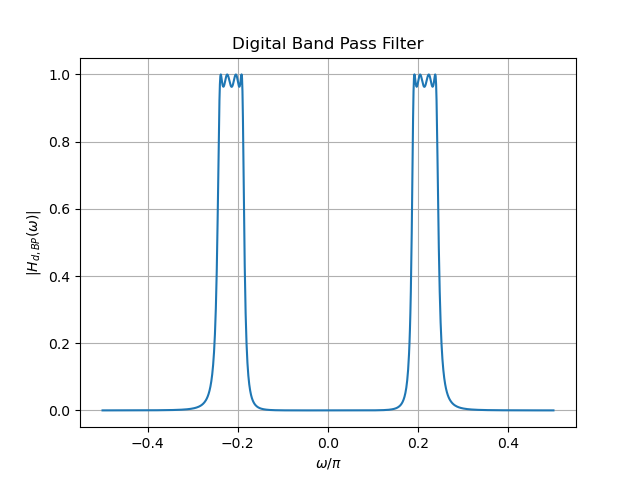
\includegraphics[width = \columnwidth]{figs/fig5}
		\centering
		\label{fig: fig5}
	\end{figure}
	
	\solution
	
	\begin{table}[ht] 
		\centering
		\input{tables/table5}
		\caption{input values}
		\label{tab: Table2021bm30}
	\end{table}
	By convolution we know that,
	\begin{align}
		y(n) = (x*h)(n) = \sum_{n=-\infty}^{\infty} x(k) \cdot h(n-k) \\
	\implies y(2) = 0.5h \brak 0 + 0.1h \brak 1 \\
	\implies y(3) = 0.4h \brak 0 + 0.5h \brak 1 
	\end{align}
	From the values in \tabref{tab: Table2021bm30}:
	\begin{align}
		y(2) = 0.5h \brak 0 + 0.1h \brak 1 &= 1 \\
		y(3) = 0.4h \brak 0 + 0.5h \brak 1 &= 0
	\end{align}
	By solving equations (4) and (5) we get,
	\begin{align}
		5 = 2.1h \brak 0 \\
	\implies h \brak 0 = \frac {5}{2.1} \\
	\therefore h \brak 0 = 2.38
	\end{align}
\end{document}